\subsection{Ficha vs Dominó}

\subsubsection{Descripción del Juego}

En este juego cada jugador tiene un tablero de tamaño $2\times 3$. El primer jugador tiene una ficha de dominó (que ocupa dos casillas con un lado en común) que puede colocar de $7$ formas diferentes, cada forma es mostrada en la figura \ref{fig:posiciones-domino}, con su respectiva etiqueta. El segundo jugador posee una ficha que ocupa una sóla casilla de su tablero y la ubica en una de las $6$ casillas, las cuales se numeran en la Figura \ref{fig:posiciones}. Luego se superponen los tableros y si la ficha es cubierta por el dominó entonces el segundo jugador gana, en caso contrario gana el primer jugador \cite[p. 237]{bib:pl-chvatal}.

\begin{figure}[hbt]
\caption{Posibles posiciones de la ficha de dominó}
\label{fig:posiciones-domino}
\centering

\includegraphics[width=1\textwidth]{figuras/posiciones-domino.png}
\end{figure}

\begin{figure}[hbt]
\caption{Posibles posiciones de la ficha del segundo jugador}
\label{fig:posiciones}
\centering

\includegraphics[width=0.4\textwidth]{figuras/posiciones.png}
\end{figure}

\begin{table}[hbt]
\begin{center}
\caption{Matriz de pagos del juego Ficha vs Dominó}
\label{table:pagos-domino}
\begin{tabular}{ c | c | c | c | c | c | c |}
  &  1 &  2 &  3 &  4 &  5 &  6 \\ \hline
A & -1 & -1 &  1 &  1 &  1 &  1 \\ \hline
B &  1 &  1 &  1 & -1 & -1 &  1 \\ \hline
C &  1 & -1 & -1 &  1 &  1 &  1 \\ \hline
D &  1 &  1 &  1 &  1 & -1 & -1 \\ \hline
E & -1 &  1 &  1 & -1 &  1 &  1 \\ \hline
F &  1 & -1 &  1 &  1 & -1 &  1 \\ \hline
G &  1 &  1 & -1 &  1 &  1 & -1 \\ \hline
\end{tabular}
\end{center}
\end{table}

El problema de programación lineal asociado es:
\begin{equation}
\begin{array}{r r r r r r r r r r r r r r r r r r}
max        &z& &   & &   & &   & &   & &   & &   & &   &      & \\
\text{s. a}
	& & &x_1&+&x_2&+&x_3&+&x_4&+&x_5&+&x_6&+&x_7& =    &1 \\
    &z&+&x_1&-&x_2&-&x_3&-&x_4&+&x_5&-&x_6&-&x_7& \leq &0 \\
    &z&+&x_1&-&x_2&+&x_3&-&x_4&-&x_5&+&x_6&-&x_7& \leq &0 \\
    &z&-&x_1&-&x_2&+&x_3&-&x_4&-&x_5&-&x_6&+&x_7& \leq &0 \\
    &z&-&x_1&+&x_2&-&x_3&-&x_4&+&x_5&-&x_6&-&x_7& \leq &0 \\
    &z&-&x_1&+&x_2&-&x_3&+&x_4&-&x_5&+&x_6&-&x_7& \leq &0 \\
    &z&-&x_1&-&x_2&-&x_3&+&x_4&-&x_5&-&x_6&+&x_7& \leq &0 \\
    & & &x_1,&&x_2,&&x_3,&&x_4,&&x_5,&&x_6,&&x_7,&\geq &0 \\
\end{array}
\end{equation}

Este problema no tiene solución única (lo que implica que el juego no tiene un equilibrio de Nash único), una solución viene dada por $(z^*, x^*_1, x^*_2, x^*_4, x^*_5, x^*_6, x^*_6, x^*_7) = (\frac{1}{3}, \frac{1}{3}, \frac{1}{3}, 0, 0, 0, 0, \frac{1}{3})$ y $(w^*, y^*_1, y^*_2, y^*_3,  y^*_4, y^*_5, y^*_6) = (\frac{1}{3}, \frac{1}{3}, 0, \frac{1}{3}, 0, \frac{1}{3}, 0)$, esta solución corresponde a la estrategia en la que el jugador $1$ elige las posiciones A, B y G con probabilidad $\frac{1}{3}$ cada una, y el jugador $2$ elige las posiciones $1$, $3$, y $5$ con probabilidad $\frac{1}{3}$ cada una.

\subsubsection{Resultados Experimentales}

El primer jugador puede garantizar una ganancia esperada de, al menos $1/3$, por lo que el segundo jugador puede garantizar no perder más de $1/3$. A diferencia de los juegos anteriores, la matriz de pagos de este juegos no es simétrica y el primer jugador tiene ventaja sobre el segundo. Además, este juego no tiene un equilibrio de Nash único. En la Tabla \ref{tab:estrategias-RPS} se observa que las estrategias obtenidas para el primer jugador le permiten obtener una ganancia esperada al menos de $0.330$, $0.326$ y $0.329$, respectivamente para los procedimientos A, B y C. Todos estos valores son menores que $1/3$, pero con una diferencia menor que $0.01$. Por otra parte el segundo jugador puede garantizar un valor esperado no menor que $-0.338$ con cualquiera de los procedimientos.

\begin{table}[hbt]
    \centering
    \begin{tabular}{c c|c|r}
        & & Estrategias & $v_1 / v_2$\\
        \hline
        \multirow{2}{*}{E.N.}
        & $\sigma_1$ & $(0.333, 0.333, 0.000, 0.000, 0.000, 0.000, 0.333)$ & $0.333$ \\
        & $\sigma_2$ & $(0.333, 0.000, 0.333, 0.000, 0.333, 0.000)$ &  $-0.333$\\
        \hline
        \multirow{2}{*}{A}
        & $\sigma_1$ & $(0.136, 0.137, 0.116, 0.118, 0.198, 0.081, 0.214)$ & $0.328$ \\
        & $\sigma_2$ & $(0.165, 0.171, 0.163, 0.166, 0.166, 0.169)$ & $-0.338$\\
        \hline
        \multirow{2}{*}{B}
        & $\sigma_1$ & $(0.121, 0.118, 0.135, 0.137, 0.214, 0.078, 0.198)$ & $0.331$ \\
        & $\sigma_2$ & $(0.157, 0.178, 0.156, 0.177, 0.157, 0.175)$ & $-0.335$\\
        \hline
        \multirow{2}{*}{C}
        & $\sigma_1$ & $(0.128, 0.128, 0.129, 0.134, 0.208, 0.073, 0.202)$ & $0.330$ \\
        & $\sigma_2$ & $(0.169, 0.165, 0.168, 0.164, 0.169, 0.165)$ & $-0.334$\\
        \hline
    \end{tabular}
    \caption{Estrategias obtenidas del juego Ficha vs Dominó}
    \label{tab:estrategias-domino}
\end{table}

La Tabla \ref{tab:resultados-domino} muestra los resultados obtenidos relacionados al tiempo y número de iteraciones de los procedimientos de este juego. El procedimiento A, regret condicional, tuvo una duración promedio de $319.179$ segundos, con un número promedio de iteraciones de $108319272.4$, obteniendo un promedio de $2.95 {\times} 10^{-6}$ segundos por iteración. Con el procedimiento B, que utiliza un vector invariante de probabilidad, se obtuvo un tiempo, número de iteraciones y tiempo por iteración promedios de $11.275$ segundos, $75250.2$ iteraciones y $1.5 {\times} 10^{-4}$ segundos por iteración, respectivamente. Por último, el procedimiento C, regret incondicional, se obtuvo un tiempo promedio de $0.237$, el número de iteraciones promedio fue de $84318.5$, obteniendo un promedio de $2.81 {\times} 10^{-6}$ segundos por iteración. 

\begin{table}[hbt]
   \scriptsize
    \centering
    \begin{tabular}{r r r | r r r | r r r}
    \multicolumn{3}{c}{A} & \multicolumn{3}{c}{B} & \multicolumn{3}{c}{C} \\ \hline
	$669.839$ & $215859538$ & $3.10 {\times} 10^{-06}$ & $4.458$ & $29721$ & $1.50 {\times} 10^{-04}$ & $0.188$ & $66700$ & $2.81 {\times} 10^{-06}$ \\
	$309.685$ & $117568373$ & $2.63 {\times} 10^{-06}$ & $9.019$ & $60333$ & $1.49 {\times} 10^{-04}$ & $0.260$ & $92401$ & $2.82 {\times} 10^{-06}$ \\
	$399.170$ & $152612646$ & $2.62 {\times} 10^{-06}$ & $3.646$ & $24338$ & $1.50 {\times} 10^{-04}$ & $0.212$ & $75674$ & $2.81 {\times} 10^{-06}$ \\
	$131.570$ & $38097125$ & $3.45 {\times} 10^{-06}$ & $12.996$ & $86898$ & $1.50 {\times} 10^{-04}$ & $0.145$ & $51776$ & $2.80 {\times} 10^{-06}$ \\
	$263.482$ & $96741015$ & $2.72 {\times} 10^{-06}$ & $4.516$ & $30170$ & $1.50 {\times} 10^{-04}$ & $0.134$ & $47862$ & $2.80 {\times} 10^{-06}$ \\
	$203.854$ & $77156602$ & $2.64 {\times} 10^{-06}$ & $15.420$ & $103021$ & $1.50 {\times} 10^{-04}$ & $0.385$ & $136950$ & $2.81 {\times} 10^{-06}$ \\
	$201.267$ & $76467409$ & $2.63 {\times} 10^{-06}$ & $17.399$ & $115935$ & $1.50 {\times} 10^{-04}$ & $0.351$ & $124882$ & $2.81 {\times} 10^{-06}$ \\
	$316.007$ & $97849871$ & $3.23 {\times} 10^{-06}$ & $17.266$ & $115056$ & $1.50 {\times} 10^{-04}$ & $0.203$ & $72315$ & $2.81 {\times} 10^{-06}$ \\
	$383.736$ & $110341861$ & $3.48 {\times} 10^{-06}$ & $12.805$ & $85532$ & $1.50 {\times} 10^{-04}$ & $0.271$ & $96438$ & $2.81 {\times} 10^{-06}$ \\
	$313.177$ & $100498284$ & $3.12 {\times} 10^{-06}$ & $15.227$ & $101498$ & $1.50 {\times} 10^{-04}$ & $0.220$ & $78187$ & $2.81 {\times} 10^{-06}$ \\ \hline
	$319.179$ & $108319272.4$ & $2.95 {\times} 10^{-06}$ & $11.275$ & $75250.2$ & $1.50 {\times} 10^{-04}$ & $0.237$ & $84318.5$ & $2.81 {\times} 10^{-06}$ \\ \hline
    \end{tabular}
    \caption{Resultados del juego Ficha vs Dominó}
    \label{tab:resultados-domino}
\end{table}

La Figura \ref{fig:regret-domino} muestra el regret incondicional con respecto al tiempo de la última corrida, para los procedimientos A, B y C. Se observa como el \textit{regret} máximo converge a cero para ambos jugadores en cada uno de los procedimientos.

\begin{figure}[hbt]
\caption{Gráficas del regret con respecto al número de iteraciones del juego Ficha vs Dominó}
\label{fig:regret-domino}
\centering
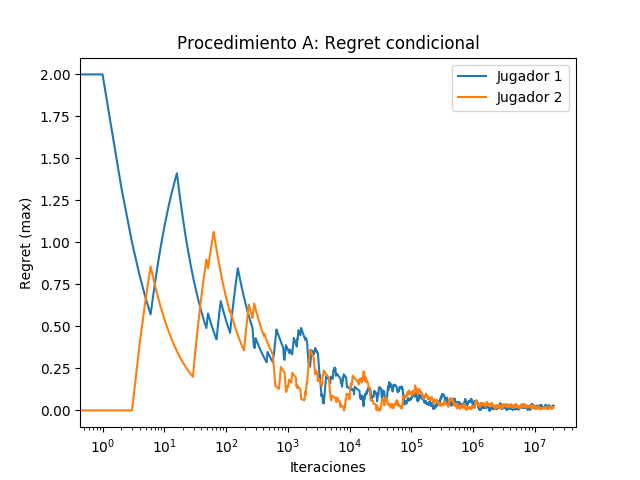
\includegraphics[width=0.45\textwidth]{graficas/domino/procedimiento-A.png}
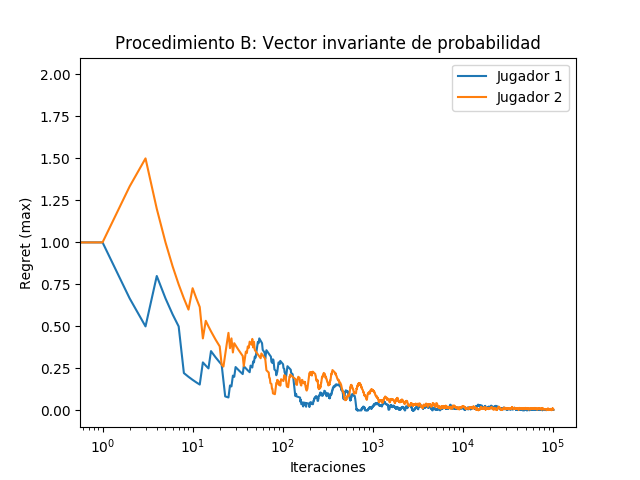
\includegraphics[width=0.45\textwidth]{graficas/domino/procedimiento-B.png}
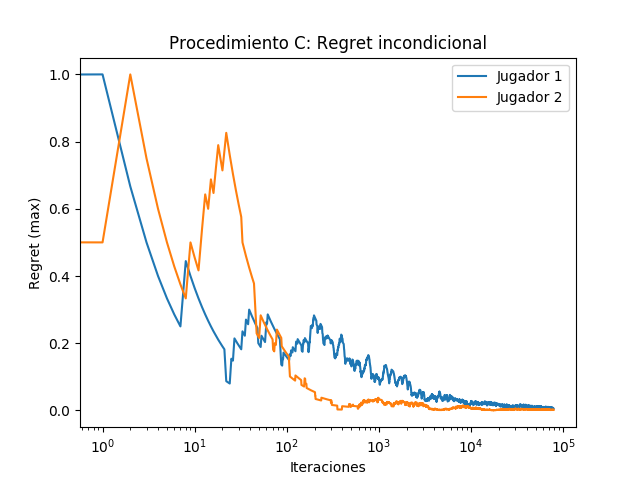
\includegraphics[width=0.45\textwidth]{graficas/domino/procedimiento-C.png}
\end{figure}
